\pagebreak
\section{Subsistema  de Estructura Mecánica} \label{subsishw}

	El subsistema Mecánico comprende la estructura tangible (estante, carcasa, armadura), en donde se realiza la activación de los dispositivos electrónicos (Hardware) y mecánicos encargados de validar y dosificar el alimento desde el tanque de almacenamiento hasta el ``plato'' de comida del novillo (comedero). Este subsistema está divido en 3 partes principales: La primera parte consta de la conexión física y mecánica de las partes que comprenden el punto de dosificación (tolva, mecanismo de dosificación, accesorios de conexión, etc). La segunda parte abarca el funcionamiento en conjunto del mecanismo de dosificación para extraer el alimento desde la tolva hasta un punto de validación de pesaje. Por último, se tiene una etapa de conexión entre el pesaje de la porción y el punto de alimentación del bovino.
	
\subsection{Análisis}
\subsubsection{Tanque de almacenamiento}
    
    De acuerdo con lo mencionado al inicio de la sección \ref{dosificadores} y retomando la estructura general de un dosificador como el de la Figura \ref{dosif2png}, es considerable que el sistema prototipo cuente con una estructura física similar. No obstante en la ganadería convencional, el alimento almacenado suele encontrarse en tanques, zonas o cuartos aislados, lejos del alcance de los animales y por lo tanto del establo de alimentación. Día a día se transportan desde estas zonas hasta los establos de alimentación, las cantidades de alimento requeridas para abastecer el ganado. Sin embargo, esto retarda la jornada diaria del proceso de ceba para grandes poblaciones de ganado.
	
	\begin{figure}[H]
		\begin{center}
			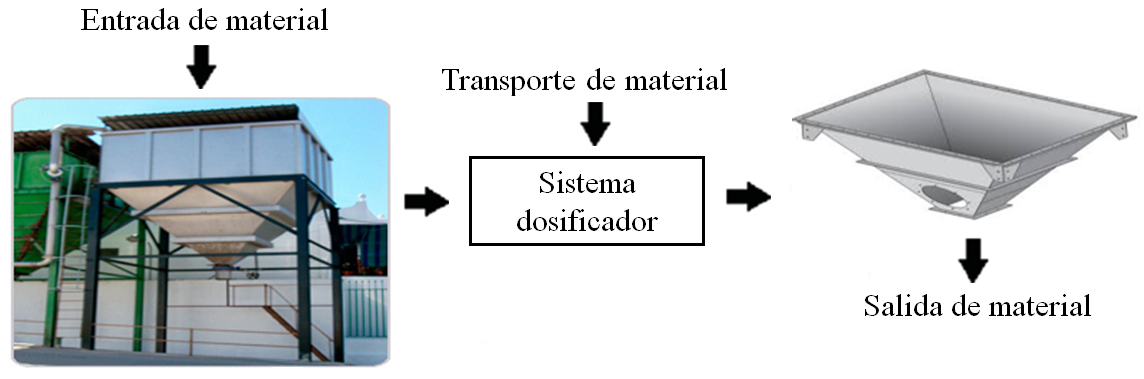
\includegraphics[scale=0.55]{img/dosificacion.png}
		\end{center}
		\caption{Estructura general de un dosificador. \label{dosif2png}}
    \end{figure}
	
	Con base en lo anterior, se plantea almacenar el alimento dietario en tanques de menor tamaño (en comparación a una habitación de almacenaje) ubicados en los establos de alimentación. De esta manera el alimento dietario puede ser re-abastecido y suministrado en un mismo lugar. Así pues, la tolva del sistema dosificador sería a su vez el tanque de almacenamiento que estaría conectado con el sistema dosificador descrito más adelante.

\subsubsection{Mecanismo de dosificación}

    Está claro que existen diferentes mecanismos usados para manipular alimentos tanto de consumo humano como animal. Estos mecanismos poseen atributos, diseños y sistemas de funcionamiento con características especializadas para su propósito; estos varían dependiendo del tipo de alimento, la cantidad de alimento, precisión, velocidad de trabajo, entre otros criterios. 
    
	Para saber cuál de estos mecanismos se acomoda a las necesidades, limitantes, situaciones y propiedades del entorno de trabajo de este proyecto, nuevamente es necesario la selección de el(los) mecanismo(s) más apropiado(s). Para ello se recurre a realizar una nueva matriz de selección con los siguientes dictámenes:
	
	\begin{itemize}
	   \item Los pesos asignados para cada criterio son valores enteros del 1 al 5.
	   \item Entre mayor sea el peso asignado, significa que la modalidad es más apropiada para cada criterio de selección.
	   \item \begin{inparaenum}[(i)]
	        Los criterios usados para esta matriz son:
	        \item ``Costo''
	        \item ``Viabilidad técnica''
	        \item ``Manipulación electrónica''
	        \item ``Precisión de Dosificación''
	        \item ``Propósito adecuado''
	    \end{inparaenum}
	    \item El criterio de costo representa la relación costo beneficio que representa cada alternativa.
	    \item El criterio de viabilidad técnica representa la posibilidad de implementación factible y apropiada para la aplicación para la cual ha sido diseñada.
	    \item El criterio de manipulación electrónica hace referencia a qué tan complejo es su uso mediante intervención electrónica. 
	    \item En cuanto al criterio de precisión, representa cuán precisa es la alternativa para la dosificación de porciones establecidas.
	    \\
    \end{itemize}

\begin{table}[H]
\centering
\caption{Matriz de selección por peso ponderado para el mecanismo dosificador. \label{matrizactpng}}
\begin{tabular}{|c|c|c|c|c|c|c|}
\hline
\multirow{3}{*}{Alternativas} & \multicolumn{5}{c|}{Criterios} & \multirow{3}{*}{\begin{tabular}[c]{@{}c@{}}Valoración \\ final de la\\  alternativa\end{tabular}} \\ \cline{2-6}
 & 25\% & 15\% & 20\% & 15\% & 25\% &  \\ \cline{2-6}
 & Costo & \begin{tabular}[c]{@{}c@{}}Viabilidad\\   técnica\end{tabular} & \begin{tabular}[c]{@{}c@{}}Manipulación\\   electrónica\end{tabular} & \begin{tabular}[c]{@{}c@{}}Precisión de\\  dosificación\end{tabular} & \begin{tabular}[c]{@{}c@{}}Propósito  adecuado\\  (manejo de alimento)\end{tabular} &  \\ \hline
\begin{tabular}[c]{@{}c@{}}Compuerta \\ deslizante\end{tabular} & 3 & 3 & 2 & 2 & 4 & 2,9 \\ \hline
\begin{tabular}[c]{@{}c@{}}Compuerta \\ rotativa\end{tabular} & 4 & 4 & 3 & 2 & 5 & 3,75 \\ \hline
\begin{tabular}[c]{@{}c@{}}Tornillo \\ sin fin\end{tabular} & 3 & 4 & 4 & 5 & 4 & 3,9 \\ \hline
\end{tabular}
\end{table}


	Teóricamente, tanto el tornillo sin fin como la compuerta rotativa poseen propósitos de dosificación de alimentos,  viabilidad técnica similar y una buena relación costo-beneficio. El factor determinante en la selección de la alternativa más apropiada es la precisión de dosificación, en la que el tornillo sin fin supera  a la compuerta rotativa. Un criterio extra en el análisis es la lejanía entre los animales y el tanque de almacenamiento. Tal y como se pudo observar en la Figura \ref{dosifpng}, el alimento se encuentra en un tanque de almacenamiento y es transportado una cierta distancia hasta el punto de alimentación del animal.
	
	Entre mayor sea esta distancia de separación, menor es el riesgo que los animales puedan llegar a tener contacto directo con el tanque. Así pues,  el mecanismo encargado de extraer el alimento será el denominado ``Tornillo sin fin''.
	Como este mecanismo es en principio mecánico, su accionamiento debe ser controlado por una señal de activación por pulsos (PWM) ocasionada por señales provenientes del subsistema ID. Por otra parte, el tornillo debe moverse rotativa y constantemente gracias a un actuador electrónico como por ejemplo un motor. \\
	
	Una vez más, es imperativo seleccionar el tipo de motor más adecuado para culminar esta tarea. Por lo que en esta ocasión los criterios decisivos serán el costo, la manipulación electrónica, el torque del motor y el consumo energético.\\
	
\begin{table}[H]
\centering
\caption{Matriz de selección por peso ponderado para el motor.} \label{matrizmotor}
\begin{tabular}{|c|c|c|c|c|c|}
\hline
\multirow{3}{*}{Alternativas} & \multicolumn{4}{c|}{Criterios} & \multirow{3}{*}{\begin{tabular}[c]{@{}c@{}}Valoración final\\   de la alternativa\end{tabular}} \\ \cline{2-5}
 & 25\% & 35\% & 20\% & 15\% &  \\ \cline{2-5}
 & Costo & Torque & \begin{tabular}[c]{@{}c@{}}Manipulación\\   electrónica\end{tabular} & \begin{tabular}[c]{@{}c@{}}Consumo\\   energético\end{tabular} &  \\ \hline
\begin{tabular}[c]{@{}c@{}}Motores\\   paso a paso\end{tabular} & 2 & 5 & 3 & 3 & 3,3 \\ \hline
\begin{tabular}[c]{@{}c@{}}Servomotores de\\  giro continuo\end{tabular} & 5 & 3 & 4 & 4 & 3,7 \\ \hline
Servomotores & 3 & 3 & 4 & 4 & 3,2 \\ \hline
\end{tabular}
\end{table}


% Observación añadida Post Sustentación el día 29 DE Julio de 2020 por comentarios del Jurado Carlos Lozano


Es esencial notar que aunque los motores paso a paso son ideales por su capacidad de torque, estos requieren de sistemas de alimentación de alta potencia, sistemas de manipulación complejos y en su mayoría son usados para controlar la posición del giro más que la velocidad de giro. Esto en otras palabras quiere decir que su accionamiento significará más tiempo de espera en la dosificación del alimento total,  ocasionando que la alta precisión de ``micro steps'' del motor paso a paso sea reemplazada por la velocidad de giro del servomotor de giro continuo.

También es imperativo recalcar que la extracción de la porción de alimento es validada y verificada por una balanza digital para corroborar que la porción de alimento que se entrega al novillo sea idealmente la deseada.

\pagebreak

\subsubsection{Tipo de Comedero}
    % \item \textbf{Tipo de Comedero}
    
    Una vez llegados a este punto el alimento ya ha sido dosificado hasta el punto de alimentación del animal. Para satisfacer el objetivo específico No. 5 sobre la detección del alimento y la ingesta de éste, se deben cumplir 2 condiciones previas. La primera, que el alimento llegue al comedero. La segunda es que el comedero se encuentre ``vacío'' nuevamente al finalizar la etapa de ingesta (ver figura \ref{dblockspng}). Esto puede corroborarse mediante sistemas de detección que pueden implementarse con diferentes sensores en conjunto con temporizadores. Para este caso, se utilizará la detección mediante sensores infrarrojos. 
    En primera instancia se piensa en posicionar los pares de emisores y receptores por niveles y considerando un comedero cilíndrico (similar al tipo canoa). Así cuando el comedero esté vacío, los infrarrojos indicarán un 0 y a medida que se llene, los n-sensores infrarrojos indicarían un valor de 1, similar a un sensor de nivel (Ver Figura \ref{infra1png}). Estos valores hacen referencia a la presencia (1) o carencia (0) de alimento.
    
    \begin{figure}[H]
	    \begin{center}
	    	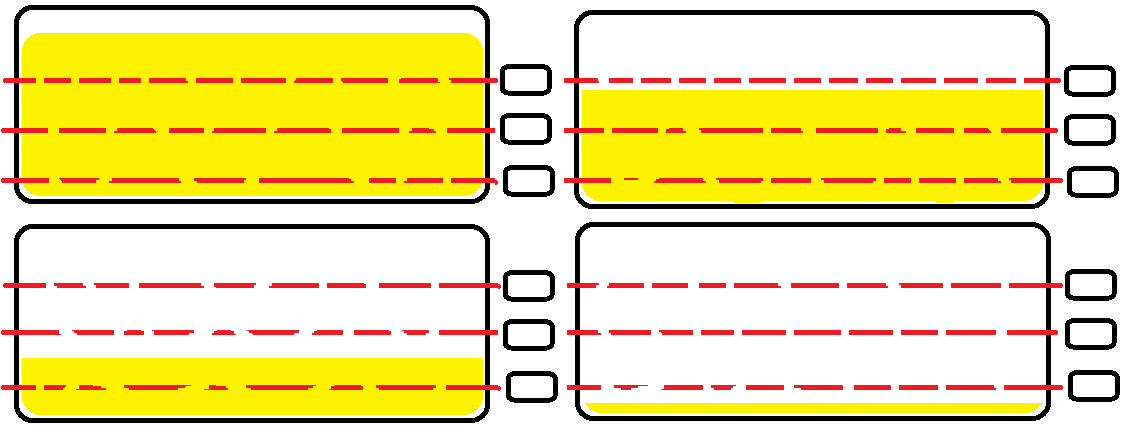
\includegraphics[scale=0.40]{img/infra1.png}
        \end{center}
	    \caption{Detección de alimento por niveles (Vista frontal del comedero).	
	    \label{infra1png}}
    \end{figure}
    
    Si el comedero se encuentra en un principio vacío (Estado de infrarrojos en 0), al momento de dosificar el alimento, los infrarrojos se encontrarán en un estado de 1. Una vez se cumpla el tiempo de espera para la ingesta del alimento, se corrobora si el estado de los sensores infrarrojos es nuevamente 0 (condición \#2).\\
    Si es así, la ingesta ha sido satisfactoria; en caso contrario se debe reportar en la base de datos y alertar inmediatamente al personal mediante un aviso correspondiente (sonoro, visual, etc). De esta manera se pueden satisfacer los objetivos específicos \#4 y \#5 al permitir la verificación de ingesta (satisfactoria/insatisfactoria) del alimento.
    
    
    
\subsection{Diseño}
% tornillo sin fin como extractor y transportador,
% El proceso de diseño para este subsistema abarca 3 partes. La primera consta de la conexión física y mecánica de las partes que comprenden el punto de dosificación. La segunda parte abarca el funcionamiento en conjunto del mecanismo de dosificación hasta el pesaje mediante la balanza digital. La última parte consta de una etapa de conexión entre el alimento pesado por la balanza y la entrega de ese alimento hasta el punto de alimentación del bovino (el plato). La tercera parte consta del diseño de la estructura física que soporta la parte tangible del sistema.\\

\subsubsection{Forma de la tolva}

En la sub-sección anterior se establece que la tolva debe ser a su vez el tanque de almacenamiento del cual se extrae el alimento, y que su ubicación debe estar en el establo de alimentación. En lo que respecta al diseño físico de este elemento, por simplicidad comercial  se opta por una tolva de forma cónica, también conocida como Silo (Ver figura \ref{tolvapng}).

\begin{figure}[H]
	\begin{center}
		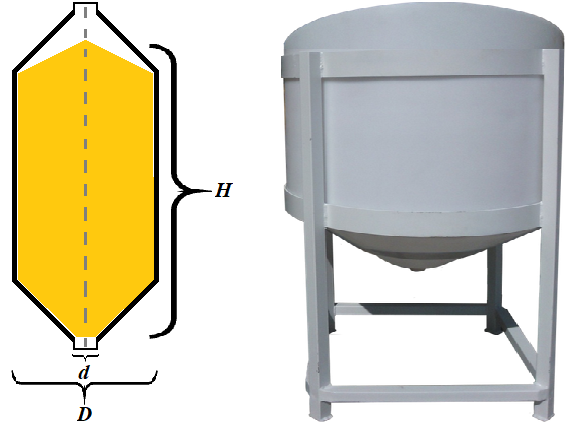
\includegraphics[scale=0.50]{img/tolvas.png}
	\end{center}
	\caption{Forma de la tolva. \label{tolvapng}}
\end{figure}

\subsubsection{Distribución de los puntos de alimentación}
Por otra parte, si se desea alimentar grupos de ganado de forma organizada y controlada, el tanque debe contar con un mecanismo tal que esté en la capacidad de abastecer a varios individuos a la vez. Para ello se diseñan puntos de alimentación en diferentes direcciones alrededor de cada tanque. De esta manera, 
%considerando las dimensiones físicas de ejemplares de esta ganadería,
se establecen hasta 4 puntos de alimentación por cada tolva instalada.
 
\begin{figure}[H]
	\begin{center}
		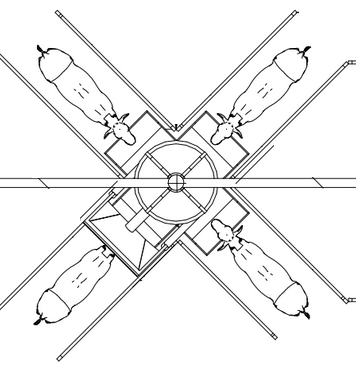
\includegraphics[scale=0.50]{img/disenotolvas.png}
	\end{center}
	\caption{Ubicación de la tolva. \label{matrizmotorpng}}
\end{figure}


% \subsubsection{Mecanismo de dosificación}

% El uso de tornillos sin fin exponen una dificultad práctica debido a su falta de disponibilidad directa en el mercado. Estos se fabrican acorde a las especificaciones del cliente, por lo tanto no es posible encontrar modelos que se adapten a las condiciones de trabajo ya establecidas. Como medida adaptativa a esta situación, se utiliza nuevamente la impresión 3D como alternativa viable para el desarrollo del prototipo y la validación del diseño que esta descrito a continuación.\\

\subsubsection{Mecanismo de extracción: Tornillo sin fin}\label{disenotorni}

Una desventaja comercial del tornillo sin fin es que solo se fabrican a la medida según la aplicación requerida; es por esto que éste debe ser diseñado con las especificaciones acordes a este proyecto para su fabricación a nivel comercial. Para hacer un diseño tentativo de éste, se realiza un modelo en 3D en SolidWorks.
%     \begin{figure}[H]
% 	\begin{center}
% 		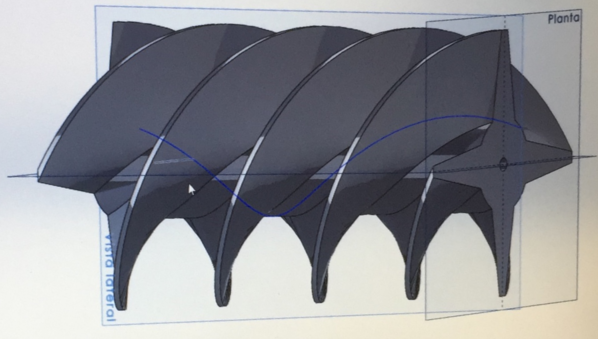
\includegraphics[scale=0.85]{img/torni3d.png}
% 	\end{center}
% 	\caption{Bosquejo 3D en SolidWorks del Tornillo sin fin. \label{torni3dpng}}
%     \end{figure}

Como se menciona en la sección \ref{endscrew}, el proceso de diseño de un mecanismo de dosificación mediante el uso de un tornillo sin fin consta de diferentes partes:

\begin{enumerate}[(1)]
    \item \textbf{Determinar el Paso ($P$), Diámetro interno ($d$) y Diámetro externo del tornillo ($D$): } Para acoplar el servomotor de giro continuo junto con el tornillo, se utiliza uno de los accesorios convencionales del servomotor (ver figura \ref{accesorioservopng}). Se utiliza este accesorio circular debido a que el tornillo consta de un diámetro interno, con eje rotativo concéntrico al eje giratorio del motor que le acciona, facilitando el acople entre ambas piezas.
    
    \begin{figure}[H]
	\begin{center}
		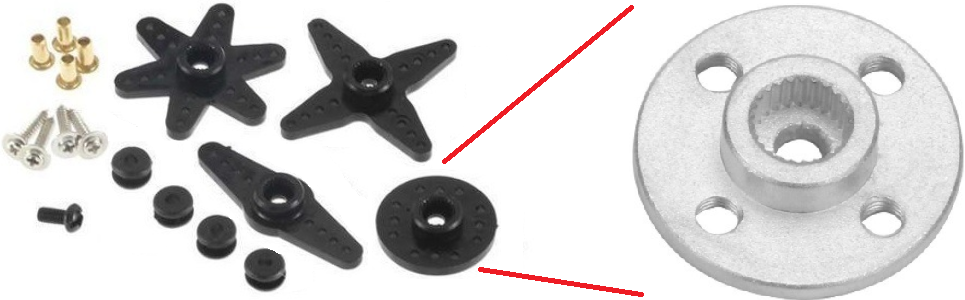
\includegraphics[scale=0.45]{img/accesorioservo.png}
	\end{center}
	\caption{Accesorios de rotación para servomotor. \label{accesorioservopng}}
    \end{figure}
    
    Este accesorio contiene 4 orificios por los que atraviesan 4 tornillos que por fricción conectan al accesorio y al tornillo. A grosso modo podría considerarse que la unión del accesorio y el tornillo conforman un accesorio más grande para el servomotor (ver Figura \ref{accesoriograndepng}).
    Para acoplar el accesorio del servo junto con el tornillo, el diámetro interno ($d$) de este último debe ser mayor o igual que el diámetro  externo del accesorio, es decir, aproximadamente una pulgada ($ 1 [inch] \approx 25,4 [mm]$).
    
    \begin{figure}[H]
	\begin{center}
		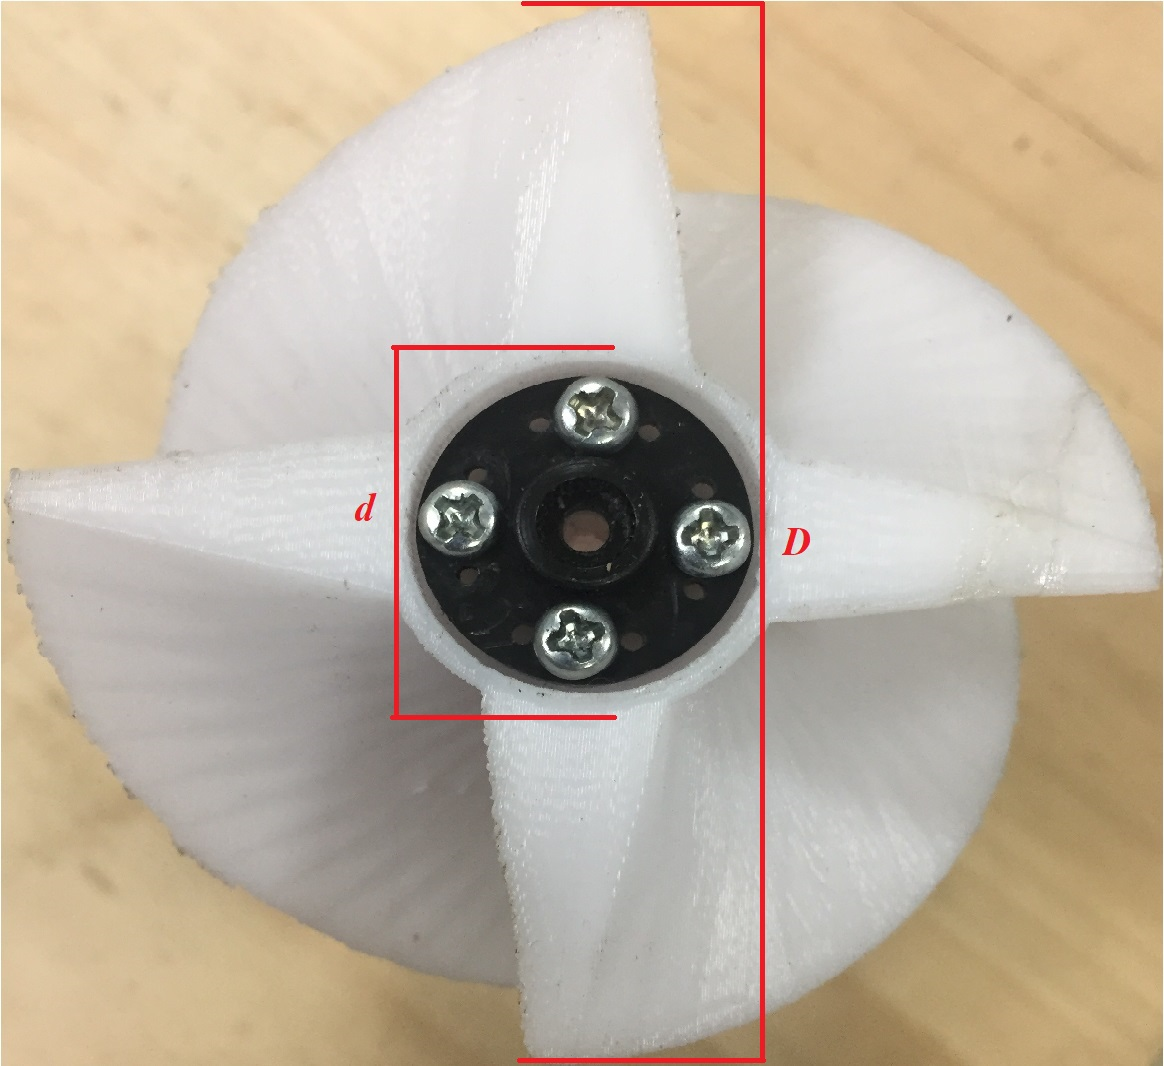
\includegraphics[scale=0.13]{img/accesoriogrande.png}
	\end{center}
	\caption{Accesorio ``tipo tornillo'' para servomotor. \label{accesoriograndepng}}
    \end{figure}
    
    Una vez establecido el diámetro interno del tornillo ($d$),  se considera por facilidad de diseño que el largo de las hélices serán de igual diámetro que $d$, dando como resultado que el Diámetro externo $D$ sea diseñado con un tamaño tres veces más grande que el interno ($ D = 3\cdot d $). No obstante, para garantizar que el tornillo girará sin inconvenientes ni roces forzosos o fricción indeseada con las paredes del canalón comercial de 3 pulgadas; se sustrae una holgura de $\pm 0,25 [mm]$ a cada lado dando como resultado que $D \approx 75 [mm]$.\\
    
    Como el material a transportar es pulverizado y semi granulado sólido, estos son considerados como materiales de buena capacidad de flujo. A su vez, las hélices deben ser continuas para garantizar el transporte continuo del material; por consiguiente basándonos en la tabla \ref{helices}, el paso ($P$) puede ser entre 1 a 2 veces el tamaño del diámetro interno $d$. Así pues, se considera un paso de igual tamaño que $d$.
    
    \item \textbf{Características del canalón y longitud del tornillo}
    
    Como ya se ha definido que el diámetro externo $D$ es $0,5 [mm]$ más pequeño que el diámetro interno del canalón, se puede confirmar que a esta nueva incógnita se le atribuye un valor de aproximadamente 3 pulgadas. Recapitulando lo explicado en la Sección \ref{endscrew}, el canalón es una superficie externa que bordea al tornillo de forma parcial o total, y a su vez hace parte de la armadura del mecanismo de dosificación.
    
    Comercialmente los tubos de PVC manejan dimensiones en pulgadas, facilitando su uso para este prototipo e incluso para aplicaciones reales. Con base en lo anterior el largo del canalón dependerá de las dimensiones comerciales de este producto.
    
    Entre las marcas más comerciales de tubería PVC están ``Pavco'' y ``Durman'', que poseen características y materiales similares. Sin embargo por motivos de limitantes económicos en este trabajo, se opta por los artículos menos costosos para las pruebas y/o modificaciones que se requieran.
    
    \begin{inparaenum}[(i)]
	        Antes de mostrar el tipo de tubería usada para representar el canalón, es imperativo observar que el canalón posee 3 aperturas de conexión hacia:
	        \item ``La tolva de almacenamiento'', mediante una boquilla de entrada de carga,
	        \item ``El motor de giro'' y por último
	        \item ``La salida del material'', mediante una boquilla de descarga.
	 \end{inparaenum}
	 
	 Con esto en mente, se opta por seleccionar una tubería tipo ``Tee'' como la que se muestra a continuación:
	 
	\begin{figure}[H]
	    \begin{center}
	    	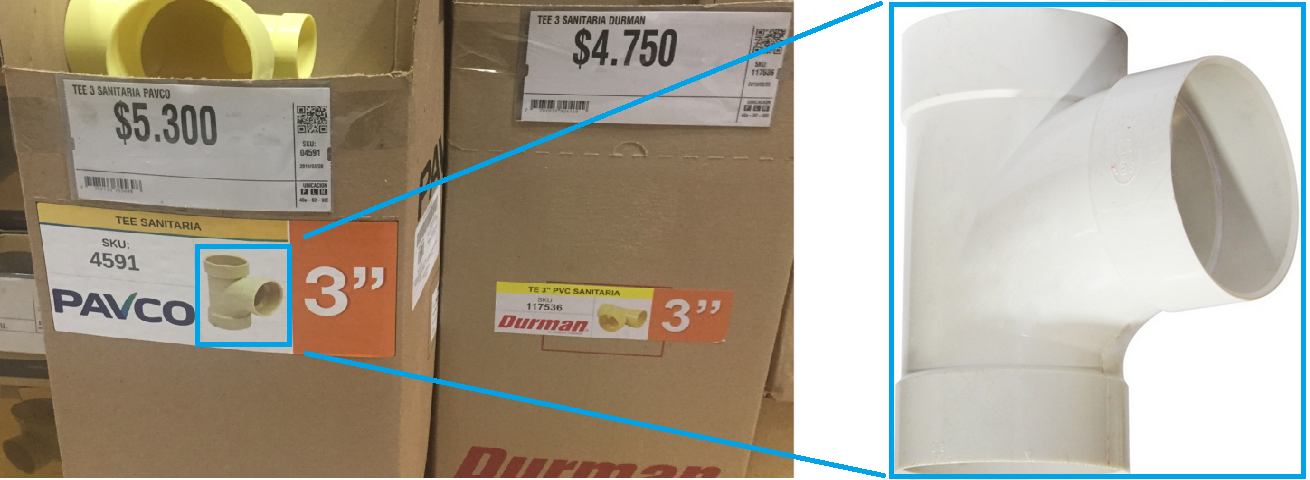
\includegraphics[scale=0.60]{img/pvct.png}
        \end{center}
	    \caption{Tubería de PVC tipo Tee. \label{pvctpng}}
    \end{figure}
	 
	De la figura \ref{pvctpng} se tiene que las aperturas opuestas conectarán con el motor y la boquilla de descarga respectivamente, mientras que la apertura restante conectará con la tolva de almacenamiento del alimento. 
	
	Antes de determinar el largo del canalón y por consiguiente el largo del tornillo, se debe agregar lo siguiente.
	
	Como la tubería de PCV tipo Tee no cuenta con una boquilla de descarga direccionada hacia abajo, se acopla un codo de ${90}^o$. Con esta añadidura se ayuda a guiar la caída del alimento pero esto requiere de una unión mediante un tubo de conexión para 3 pulgadas que ocasiona el alargamiento de la longitud final del canalón. 
% 	(ver figura 321654987). 
	
	En lo que respecta al extremo que conecta con el motor, se considera apropiado que para protegerlo y disminuir su exposición con el entorno, éste debe estar dentro de la armadura del sistema dosificador. De esta manera se añade un ``Adaptador para limpieza'' que conecta con la Tee sin necesidad de tubos de conexión (ver Figura \ref{adaptador3ppng}) y que además posee una tapa hermética que puede enroscarse y desenroscarse para acceder al motor en caso de reparaciones, manipulaciones, mantenimiento y limpieza en el futuro.
	
	\begin{figure}[H]
	    \begin{center}
	    	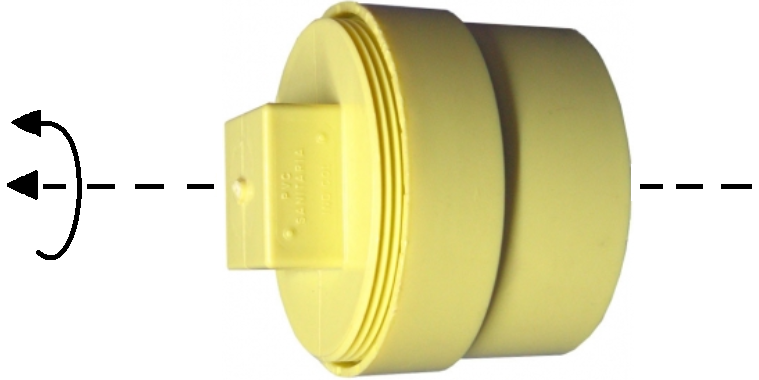
\includegraphics[scale=0.45]{img/adaptador3p.png}
        \end{center}
	    \caption{Adaptador para limpieza de PVC. \label{adaptador3ppng}}
    \end{figure}
	
	\pagebreak
% 	De igual forma para la apertura de conexión con el motor, se
    Finalmente se obtiene un canalón  compuesto  por el adaptador de limpieza, un tubo de conexión de $3"$, un codo de ${90}^o$ y la Tee de reducción de $3"$ a $2"$; que al unirlos  se obtiene que el canalón posee una longitud aproximada de $30 [cm]$.
    
    \begin{figure}[H]
	    \begin{center}
	    	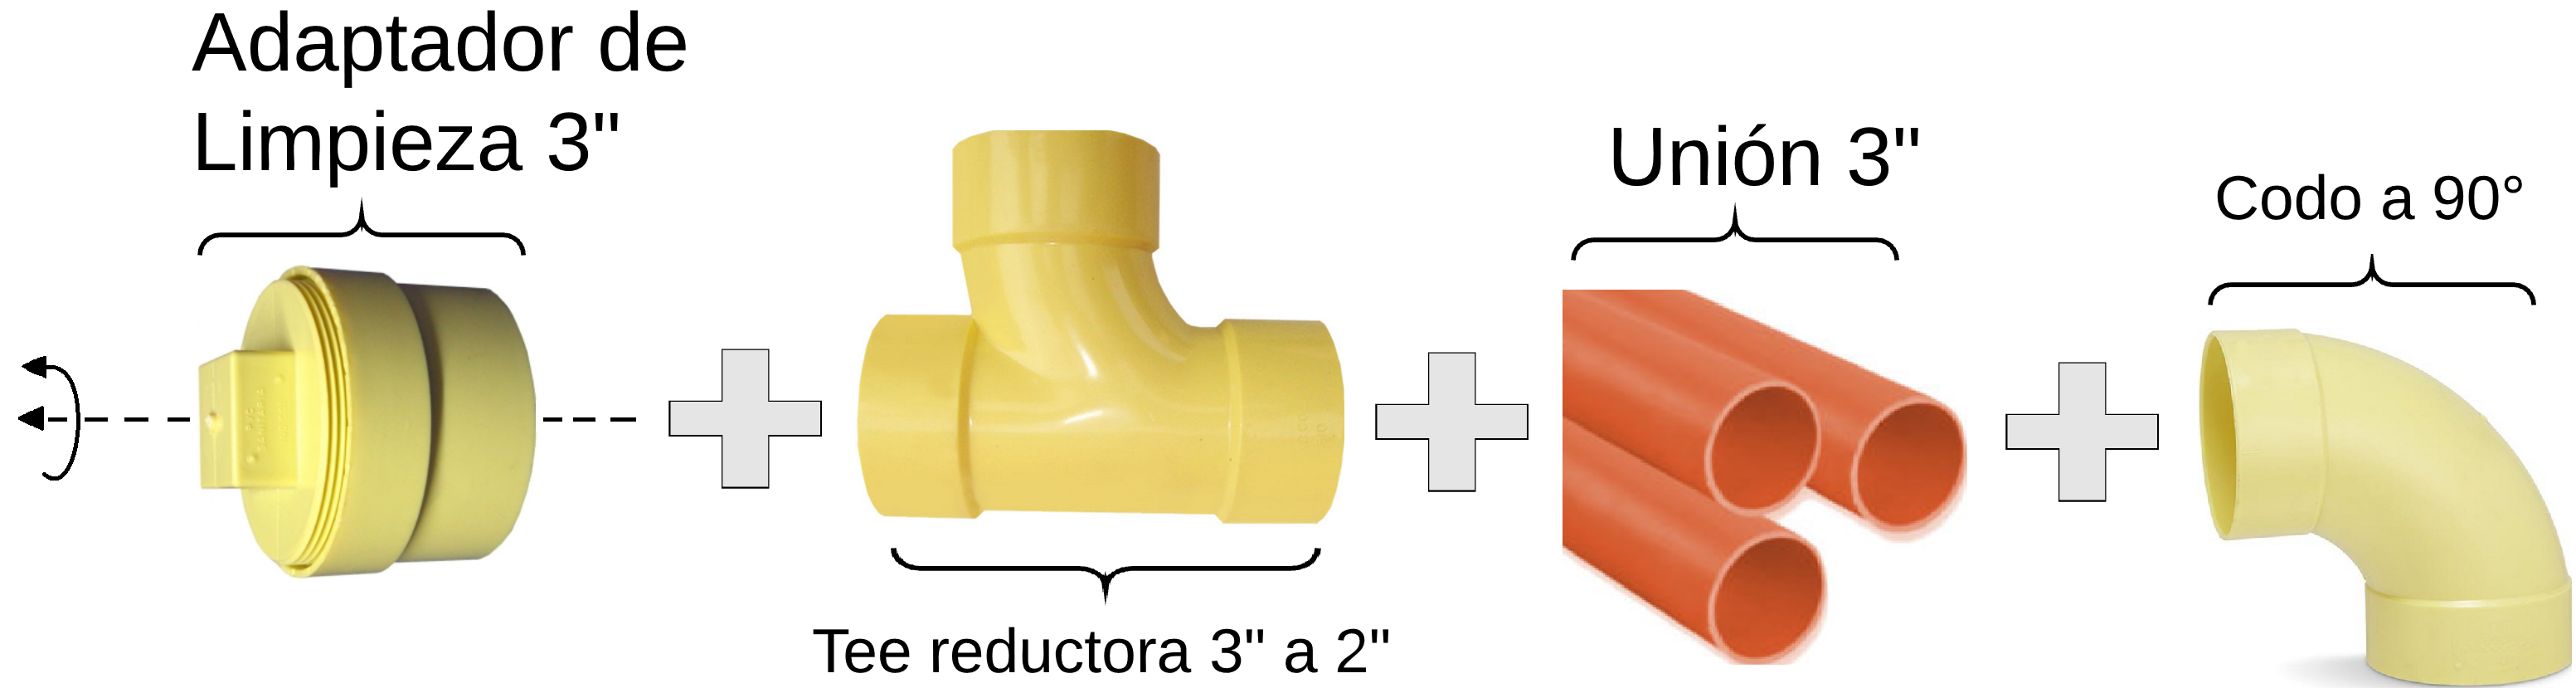
\includegraphics[scale=0.21]{img/canalontotal.png}
        \end{center}
	    \caption{Longitud total del Canalón. \label{adaptador3ppng}}
    \end{figure}
    
    Así pues, el tornillo al estar contenido dentro del canalón y al estar acoplado al motor de giro, poseerá una longitud menor a la longitud total del canalón. Se espera diseñar un Tornillo sin fin de $250[mm]$.\\
    
    \item \textbf{Diseño mecánico del tornillo sin fin}
    
    El diseño del tornillo parte del modelado en 3D. Este se realiza mediante la herramienta SolidWorks para el diseño, bosquejo, modelado y posibles modificaciones.
    Se parte del croquis de una superficie plana que será revolucionada para conformar un objeto final en 3D. Para esto, es importante establecer el número de hélices para dibujarlas en el croquis principal del transportador. En este caso, el tornillo será de $250[mm]$, por lo que se opta por tener 4 hélices equidistantes, de esta forma el croquis principal del tornillo obtiene la siguiente forma:
    
    \begin{figure}[H]
	    \begin{center}
	    	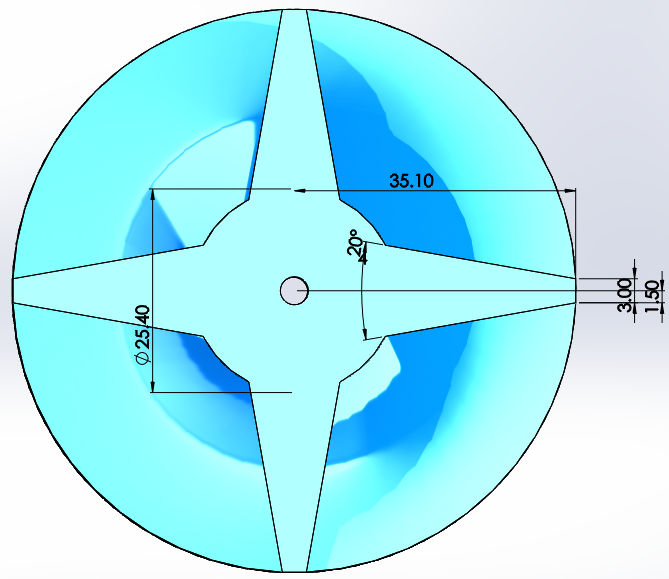
\includegraphics[scale=0.35]{img/croquisppal.png}
        \end{center}
	    \caption{Croquis principal del Tornillo sin fin. \label{croquisppalpng}}
    \end{figure}
    
    De esta forma, por cada revolución o vuelta completada por el tornillo se otorgarán 4 micro-dosificaciones (idealmente) de igual cantidad.
    Una vez definido el Croquis principal, se procede a utilizar la función de ``Barrido de saliente base'', con la que se revoluciona el croquis 2D conformando así el objeto 3D:
    
    \begin{figure}[H]
	    \begin{center}
	    	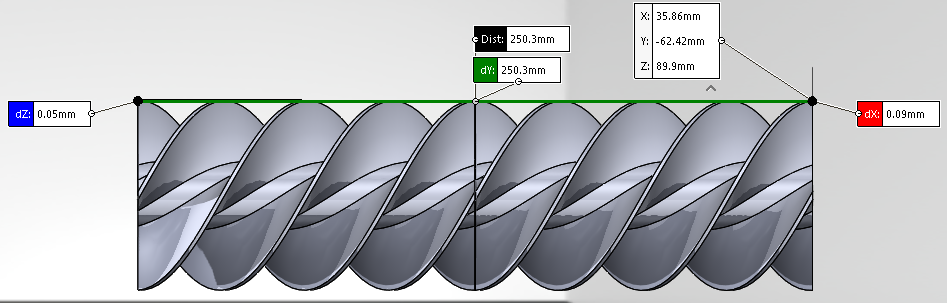
\includegraphics[scale=0.55]{img/largotorni.png}
        \end{center}
	    \caption{Primer Modelado de tornillo sin fin. \label{largotornipng}}
    \end{figure}
    
    \textbf{Obs: } Como se puede observar en la Figura \ref{croquisppalpng}, el tornillo diseñado cuenta con un orificio cuyo eje de rotación es concéntrico al eje de giro del motor y es por medio de este que se realiza el ajuste entre estas 2 partes. Para la elaboración del prototipo, se ajustará el accesorio ``Tornillo'', al espacio del motor de giro continuo mediante un tornillo de tipo M3 (ver figura \ref{torniservopng}).
    
    \begin{figure}[H]
	    \begin{center}
	    	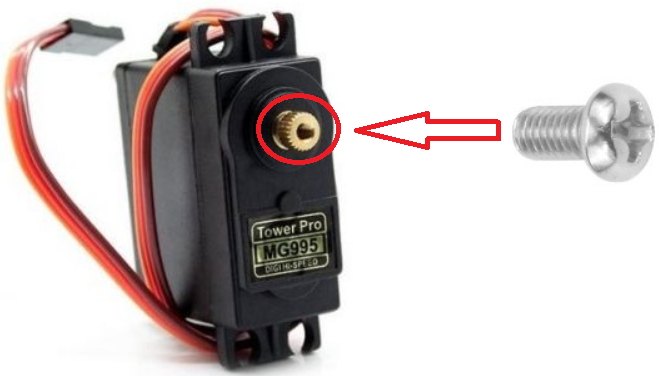
\includegraphics[scale=0.40]{img/torniservo.png}
        \end{center}
	    \caption{Tornillo de acople para accesorios del Servomotor. \label{torniservopng}}
    \end{figure}
    
    \end{enumerate}  % -------------------------------------------------------------
    \pagebreak
    \subsubsection{Mecanismo de  dosificación: Escobillas de barrido} \label{escobillas}
    
    Una vez finalizada la extracción de alimento y corroborado su peso, se debe trasladar el alimento desde la superficie de la balanza hasta la superficie del puesto de comida o en palabras técnicas, el comedero. Para ello se pensó en acoplar la balanza, a un mecanismo de giro que incline la misma y deje caer el alimento por gravedad (ver figura \ref{girobalanzapng}).
    
    \begin{figure}[H]
	    \begin{center}
	    	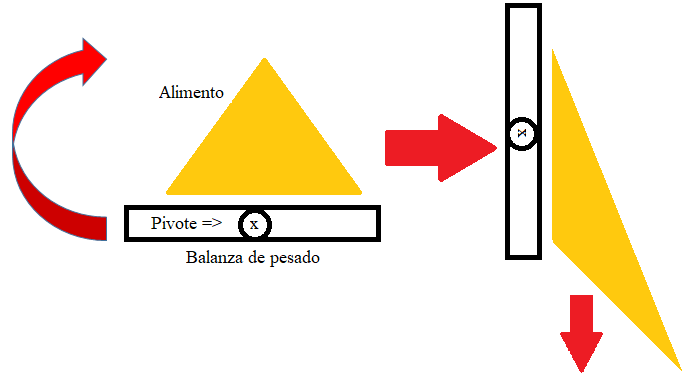
\includegraphics[scale=0.60]{img/girobalanza.png}
        \end{center}
	    \caption{Giro de la balanza. \label{girobalanzapng}}
    \end{figure}
    
    No obstante, el diseño comercial de las balanzas digitales posiciona la celda de carga de forma que el punto de presión esté en el extremo que hace contacto con la superficie de apoyo (mesa, piso) y no con la superficie que hace contacto directo con el material. Por lo tanto, si la presión ejercida sobre la balanza supera la presión soportada por el eje de giro usado para el movimiento rotativo de la balanza, no se podría realizar la inclinación de la balanza y el alimento no llegaría al plato de comida.  Como resultado, se opta por utilizar otra solución que satisfaga este último paso.
    
    Aunque los motores puedan usarse para mover objetos de forma lineal (directa o indirectamente), el movimiento básico de todo motor es el movimiento rotacional. Con base en esto se propone aprovechar esta característica para desplazar el alimento de la superficie de la balanza mediante escobillas de barrido que ``barran'' el alimento de la balanza. Así, si estas escobillas se encuentran acopladas a un motor de giro continuo, podrán barrer la porción de comida de manera continua. El diseño de esta pieza constará de 2 extremos que tendrán unida una superficie plana  para desplazar el alimento (en 1 y 2, Figura \ref{barredorespng}).

    \begin{figure}[H]
	    \begin{center}
	    	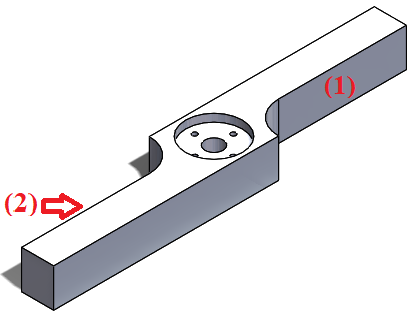
\includegraphics[scale=0.50]{img/barredores.png}
        \end{center}
	    \caption{Superficies para conexión de escobillas. \label{barredorespng}}
    \end{figure}
    
    En su centro se requiere de una hendidura para acoplarla con el motor de giro continuo al igual a como se hizo para el acople del tornillo sin fin (Ver Figura \ref{acopleservopng}).

    \begin{figure}[H]
	    \begin{center}
	    	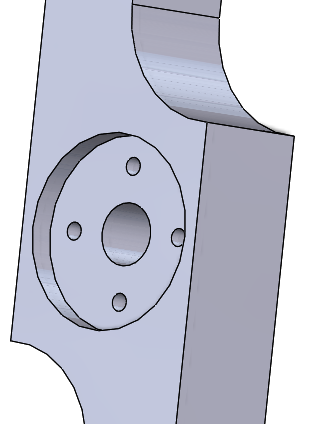
\includegraphics[scale=0.45]{img/acople_servo.png}
        \end{center}
	    \caption{Hendidura de acople para motor. \label{acopleservopng}}
    \end{figure}

    El diseño de un (1) accesorio de barrido se puede apreciar en la Figura \ref{vistasbarredorpng}, donde se puede observar  sus dimensiones en la vista inferior, seguido de la vista superior.
    
    \begin{figure}[H]
	    \begin{center}
	    	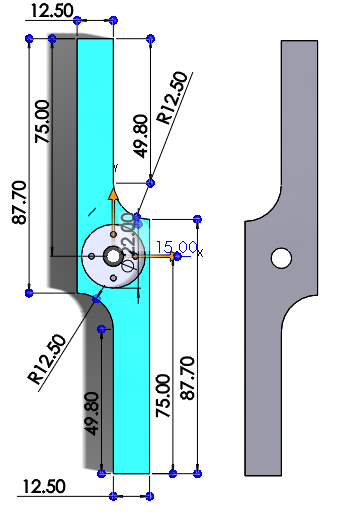
\includegraphics[scale=0.50]{img/vistasbarredor.png}
        \end{center}
	    \caption{Vistas Inferior, Superior del accesorio. \label{vistasbarredorpng}}
    \end{figure}

    Para garantizar el desplazamiento del alimento se hace uso de 2 motores a los lados de la balanza  y cada uno contará con una escobilla que al girar asincrónicamente desplazarán el alimento. 
    
     %---------------------------------------------------------------------------

    
    \subsubsection{Tipo de Comedero y detección de alimento}  \label{detectcomedero}

    Procediendo con el análisis previo de este ítem, si los sensores se ubican en una sola posición del plato se pueden presentar ocasiones en las que el alimento consumido se agrupe al extremo opuesto del sensor y se considere que el alimento ha sido ingerido satisfactoriamente cuando en realidad no es así (ver Figura \ref{infra2png}).

    \begin{figure}[H]
	    \begin{center}
	    	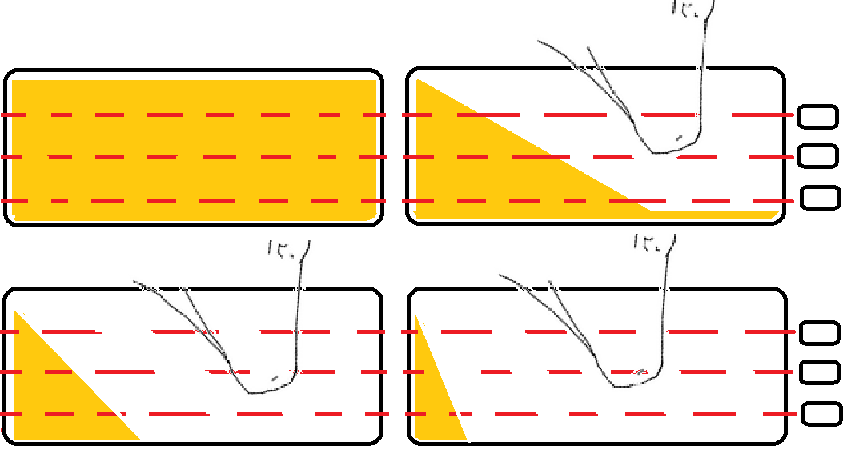
\includegraphics[scale=0.50]{img/infra2.png}
        \end{center}
	    \caption{Problema de detección \#1. \label{infra2png}}
    \end{figure}

    Como medida correctiva se opta por re-posicionar los infrarrojos en la base del plato, en forma de grilla circular, tratando de abarcar toda la superficie del comedero. No obstante se puede dar el caso que la grilla no abarque toda la superficie y se sigan presentando errores por no abarcar toda la superficie.
    % (ver vistas lateral y superior del comedero en la Figura \ref{infra3png}).

    \begin{figure}[H]
	    \begin{center}
	    	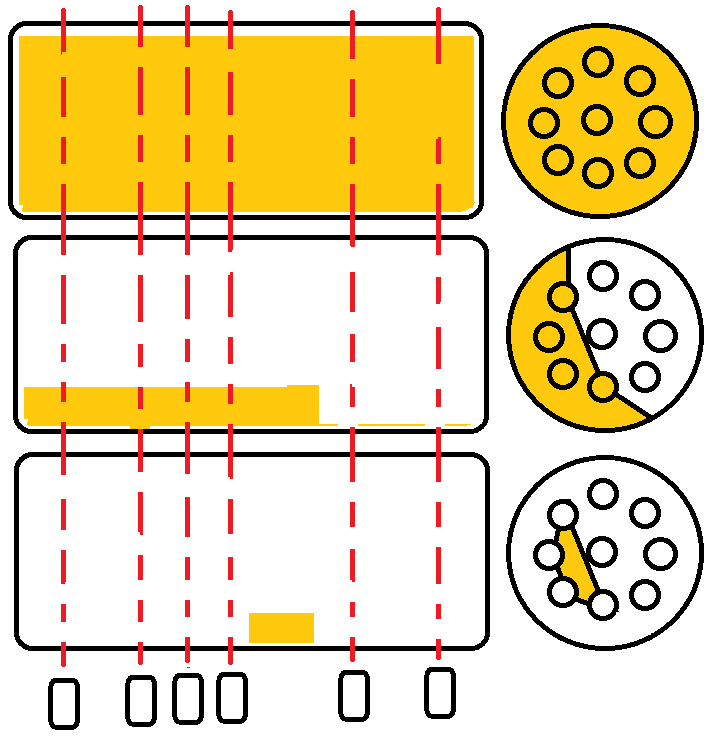
\includegraphics[scale=0.45]{img/infra3.png}
        \end{center}
	    \caption{Problema de detección \#2. \label{infra3png}}
    \end{figure}

    Así pues como última medida se opta por usar un comedero con detección vertical. De esta forma, a medida que el alimento es ingerido por el animal, éste seguirá cayendo por gravedad, así pues la grilla solo deberá ser posicionada en el extremo inferior del plato reduciendo el área de detección (Ver Vista lateral en la Figura \ref{infra4png}).
    
    \vspace{-200}
    
    \begin{figure}[H]
	    \begin{center}
    	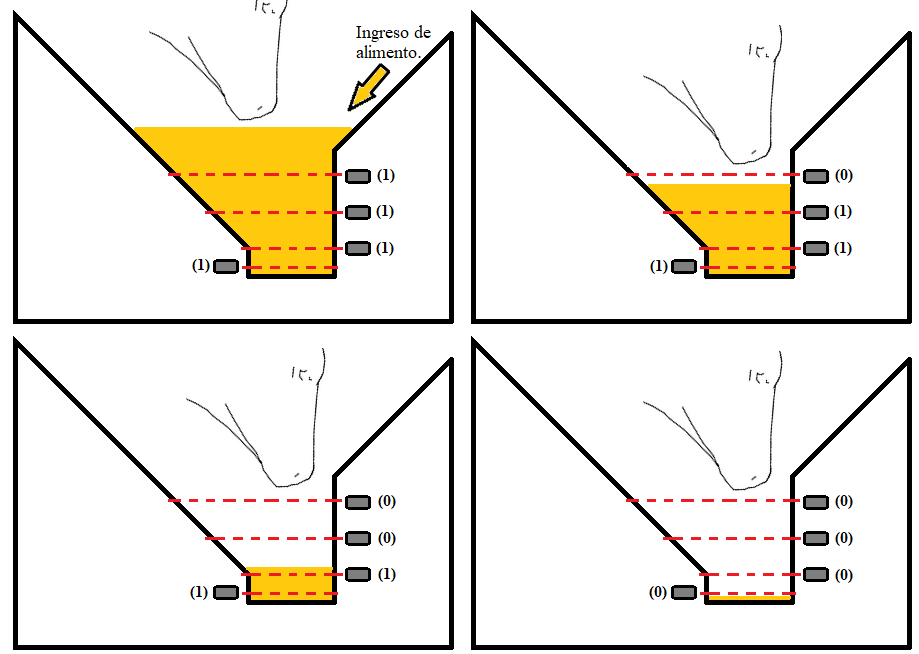
\includegraphics[scale=0.75]{img/infra42.png}
        \end{center}
	    \caption{Detección vertical de alimento en el comedero. \label{infra4png}}
    \end{figure}
    \pagebreak
    
    % \sout{hablar del diseño del suspensor del motor y de las escobillas como parte de la extracción y el pesado de alimentos y lo último de sistema de hardware hablar del plato y los infrarojos para detectar si comio o no el bovino y ahi acabo la seccion 5.3} (eso sin incluir al parte tangible la mesa, aunque eso creo que es mas un plus que algo imprescindible de hacer o de mencionar en el documento).
    
    % \textbf{Me falta cambiar las imágenes, caption y descripciones de las imagenes infra1,2,3 y 4} y paso al subsistema de sensores SECTION 5.4
    % \textbf{Me falta Agregar lo del tanque de almacenamiento y poner la figura uniones pvc que e sla que tiene todo el diagrama completo}
   
    
    % Improvise, Adapat, Overcome :)
    
    
   
    
    % ============================================
    % ============================================
    
    
     % Una vez llegados a este punto se procede a realizar la impresión 3D del tornillo en una de las impresoras 3D del CAP de la PUJ. No obstante se presentaron las siguientes dificultades:
    
    % \begin{itemize}
    %     \item La bandeja de impresión de las impresoras 3D del CAP solo imprime objetos de dimensiones menores a $140[mm]$.
    %     \item La longitud del tornillo diseñado supera esas dimensiones.
    %     \item El tiempo de impresión supera las 24 horas.
    %     \item El material requerido para hacer la impresión supera el monto autorizado para estudiantes de la carrera.
    % \end{itemize}
    
    % Estas limitaciones implican un rediseño del tornillo para que pueda ser impreso por lo que se toman las siguientes medidas:
    
    % \begin{itemize}
    %     \item El tornillo constará de 2 partes que al unirse conformarán el tornillo en su totalidad.
    %     % iguales que serán conectadas por 
    %     \item El diseño será modificado para que gaste menos material de impresión
    %     \item Al constar de diferentes piezas mas pequeñas se reduce el tiempo de impresión por pieza, ajustándose a la demanda de impresión del CAP.
    %     \item La longitud del tornillo será igual, pero las piezas que lo conforman tendrán dimensiones menores a $140[mm]$.
    % \end{itemize}
    
    
    % Retomando la figura \ref{accesoriograndepng}, el diseño de uno de los extremos del tornillo debe contener los orificios necesarios para realizar el acople entre el servo y el tornillo. Este diseño se puede apreciar a continuación:
    
    % \begin{figure}[H]
	   % \begin{center}
	   % 	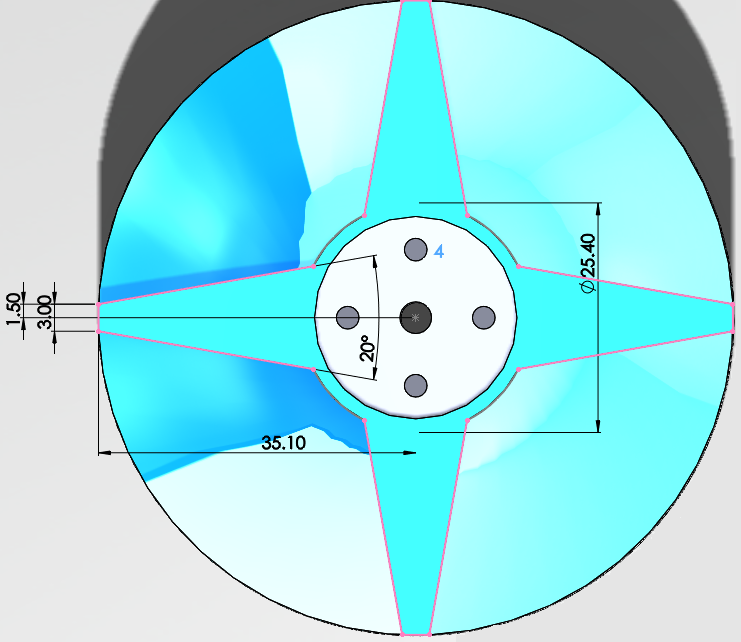
\includegraphics[scale=0.5]{img/motornillo.png}
    %     \end{center}
	   % \caption{Diseño del extremo del Tornillo que conecta con el servo motor. \label{motornillopng}}
    % \end{figure}
    
    
    % Ahora bien, dado que el tornillo constara de 2 partes, se debe considerar el modo de conexión. Para ello se opta por diseñar una parte tipo ``Macho'' y otra parte tipo ``Hembra''. De esta forma, el tornillo completo estaría formado por la conexión a presión de ambas partes.
    
    % \begin{figure}[H]
	   % \begin{center}
	   % 	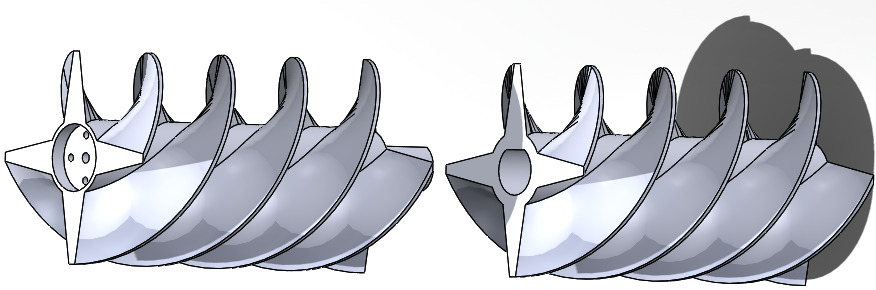
\includegraphics[scale=0.6]{img/semicircular.png}
    %     \end{center}
	   % \caption{Unión entre tornillos tipo ``Hembra'' y tipo ``Macho''. \label{semicircularpng}}
    % \end{figure}
    
    % Se había pensado que con la saliente semicircular del tornillo Macho sería suficiente para transmitir de manera apropiada el torque desde el servo hasta el extremo del tornillo. No obstante, el tornillo se ``desacoplaría'' en las condiciones en que el tornillo esté en su máxima capacidad de transporte, es decir cuando el tornillo este transportando alimento desde su inicio hasta su fin. 
    
    % De esta forma se concluye que no se ejerce fricción suficiente entre las paredes internas del tornillo que bordean la saliente del tornillo Macho y de esta forma no se transmitiría de manera apropiada el torque desde el servo hasta el extremo final del tornillo.
    
    % Con base en lo anterior, se concluye que es necesario el uso de una $3^{er}$ pieza de conexión. Esta pieza deberá tener superficies planas que ayuden a la transmisión de torque. Por otra parte debe estar separado de ambos extremos por efectos de impresión y de calentamiento del material.\\
    
    
    % Siguiendo este orden de ideas, se resume lo siguiente:
    % \begin{itemize}
    %     \item El tornillo constará de 2 partes.
    %     \item La primera que conecta el servo junto con un extremo del tornillo
    %     \item La segunda que conecta, mediante una pieza extra, las 2 partes del tornillo.
    %     \item Ambas partes del tornillo serán de tipo ``Hembra''.
    %     \item La pieza de conexión contará con 2 orificios que servirán para pasar un seguro que mantendrá firme el acople de las 2 partes de tornillos con la pieza de conexión. (ver figura \ref{piezaconexionpng})
        
    %     \begin{figure}[H]
	   %     \begin{center}
	   % 	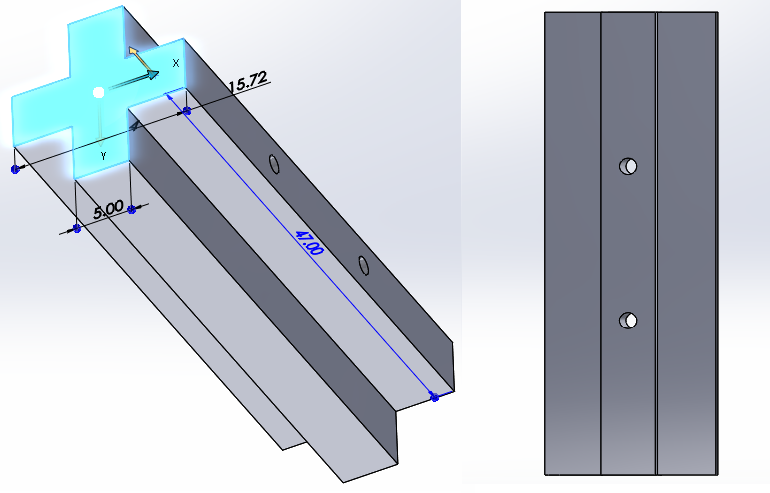
\includegraphics[scale=0.5]{img/piezaconexion.png}
    %         \end{center}
	   %     \caption{Pieza auxiliar para conexión del Tornillo. \label{piezaconexionpng}}
    %     \end{figure}
        
    %     \item Ambas piezas de tornillo tipo Hembra tendrán un orificio sobre el eje principal basados en el ítem anterior.
    % \end{itemize}
    
    % En este punto se podría cuestionar la estructura interna del tornillo debido a la dificultad visual para asimilar el diseño del tornillo. Para ello se muestra el siguiente corte trasversal de la pieza de tornillo Hembra que conecta  con el servomotor (ver figura \ref{cortetrasversalpng})
    
    % \begin{figure}[H]
	   % \begin{center}
	   % 	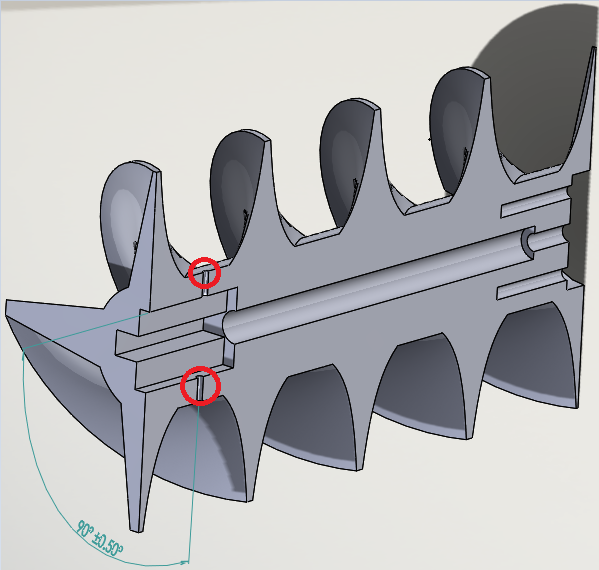
\includegraphics[scale=0.55]{img/cortetrasversal3.png}
    %     \end{center}
	   % \caption{Corte trasversal pieza tipo Hembra. \label{cortetrasversalpng}}
    % \end{figure}
    
    % \vspace{1mm}
    
    
    % En el lado izquierdo de la figura \ref{cortetrasversalpng} se puede observar el espacio para unir la pieza de conexión y el seguro. En la parte media de la figura se puede observar el corte interno del tornillo por donde pasa el atornillador que fija el tornillo M3 al servo. Por último, en el lado derecho se observa los 4 orificios para atornillar el accesorio circular del servo a la pieza del tornillo. \\
    
    % Adicionalmente se puede observar la vista superficial de esta pieza tipo Hembra en la figura \ref{vistainternapng}.
    
    % \begin{figure}[H]
	   % \begin{center}
	   % 	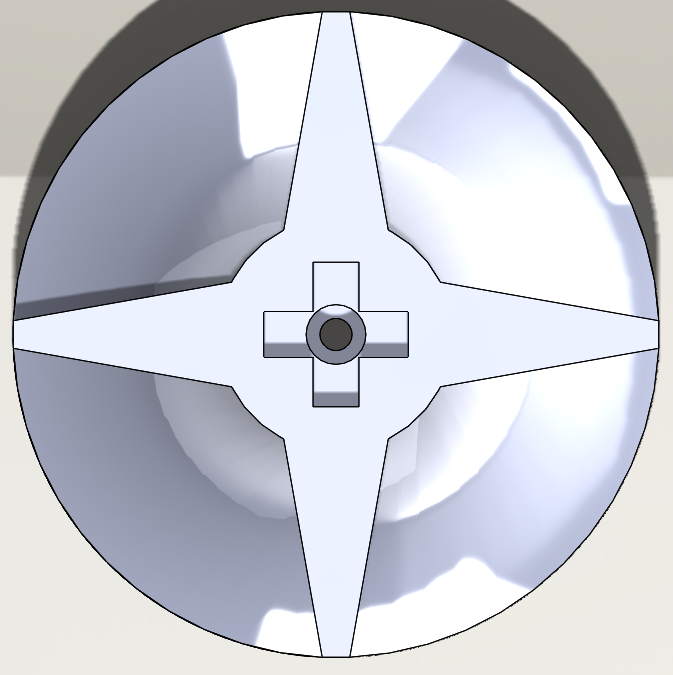
\includegraphics[scale=0.5]{img/vistainterna.png}
    %     \end{center}
	   % \caption{Vista interna de pieza tipo Hembra. \label{vistainternapng}}
    % \end{figure}
    
    % La composición final del tornillo consta del ensamblaje de las 2 piezas tipo hembras y el conector tipo cruz. el ensamblaje se logra al unir estas piezas como lo indica la figura \ref{ensambletornipng}:
    
    % \begin{figure}[H]
	   % \begin{center}
	   % 	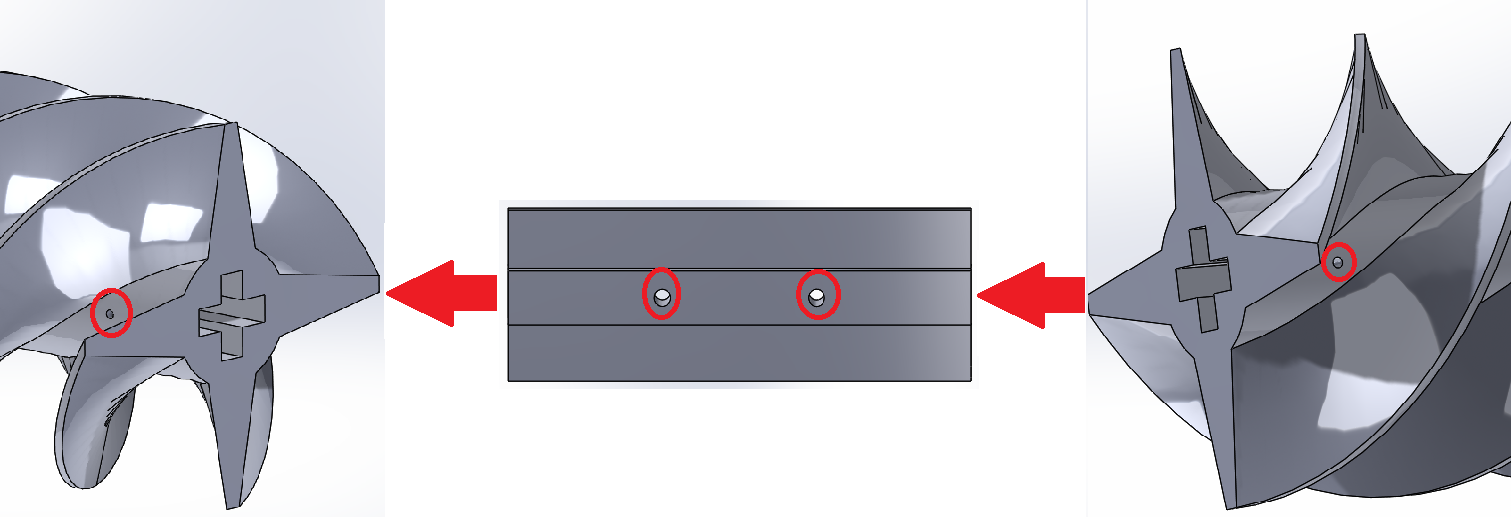
\includegraphics[scale=0.35]{img/ensambletorni.png}
    %     \end{center}
	   % \caption{Ensamble del tornillo. \label{ensambletornipng}}
    % \end{figure}
    

    % \item \textbf{Pesaje de porción: }
    
    % En lo que respecta al pesaje de la porción de alimento se ha preestablecido que ésta sería pesada a medida es extraída del tanque de almacenamiento para corroborar la cantidad ($en gramos$) que se entregará al bovino correspondiente. Para ello se requiere de una herramienta que permita medir peso. Los sensores especializados para este tipo de mediciones son las galgas extensométricas o las celdas de carga (ver figura \ref{celdaspng}). Mediante estas, se puede medir la presión que ejerce un objeto sobre una superficie y de esta forma se puede calcular la masa ([$g,kg,...$]) del objeto.
    % \begin{figure}[H]
	   % \begin{center}
	   % 	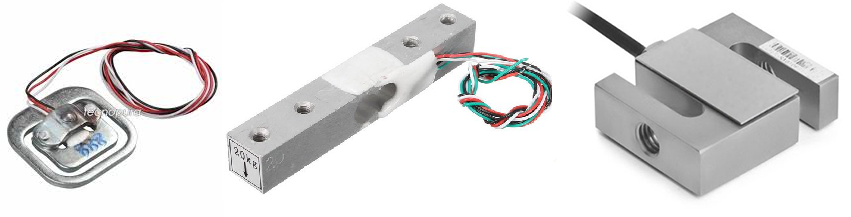
\includegraphics[scale=0.80]{img/celdas.png}
    %     \end{center}
	   % \caption{Celdas de carga y galga extensométrica. \label{celdaspng}}
    % \end{figure}
    % Estos dispositivos requieren de un acondicionamiento de la señal mediante un puente de ``Wheastone'' y de un sistema mecánico que permita distribuir la fuerzas de manera proporcional sobre toda la superficie de contacto. Además, para entregar los datos de manera digital se requiere de una etapa de conversión por medio de un ADC.
    % No obstante, en cuestión de recursos económicos, tiempo y facilidad de uso, resulta más fácil utilizar una balanza digital comercial que fabricar una balanza desde cero. De esta forma se puede aprovechar el diseño mecánico y la ubicación del sensor y solo resta transformar la señal analógica a digital.  Para esta última tarea, se utiliza el chip HX711 que  incluye el puente de ``Wheastone'' junto con una etapa de amplificadora y el ADC simplificando significativamente la inclusión de circuitería. 
    
    % A modo general, la etapa encargada de pesado el alimento extraído del tanque se observa en la figura \ref{pesajepng}:
    
    % \begin{figure}[H]
	   % \begin{center}
	   % 	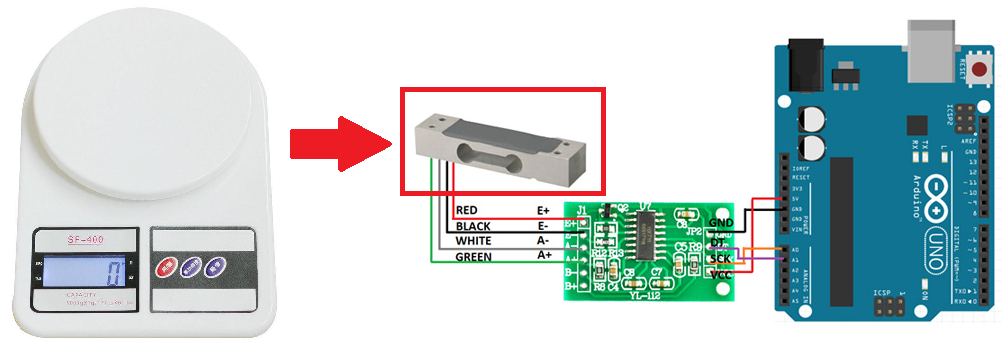
\includegraphics[scale=0.70]{img/pesaje.png}
    %     \end{center}
	   % \caption{Medición general del peso. \label{pesajepng}}
    % \end{figure}
    
    % ============================================
    % ============================================
    